\documentclass[conference]{IEEEtran}
\usepackage{graphicx}
\usepackage{booktabs}
\usepackage{amsmath,amssymb}
\usepackage{url}
\usepackage{xcolor}
\usepackage[hidelinks]{hyperref}
\usepackage{microtype}

\newcommand{\remedy}[1]{\textsc{#1}}
\newcommand{\age}{a}
\newcommand{\del}{d}

\begin{document}

\title{When Is It Too Late to Squeeze?\\
Remedy-Specific Recovery Deadlines under Observation Age and Response Delay}

\author{\IEEEauthorblockN{Nila Karthikesan}
\IEEEauthorblockA{Independent research\\
\url{https://github.com/nilakarthikesan/grasp-recovery-under-delayed-feedback}}}

\maketitle

\begin{abstract}
A runtime monitor can detect an impending grasp failure accurately and still be useless if, by the time its command takes effect, no available remedy can change the outcome. We measure how the value of three bounded recovery actions---slowing transport, squeezing to the actuator bound, and placing the object down to regrasp---depends jointly on the age of the observation the supervisor saw, the delay before its command acts, and hidden object mass, friction and an exogenous push. In a MuJoCo grasp--lift--transport--place task with a force-limited parallel-jaw gripper, we save the complete executing system at every control step after acquisition and run every remedy after every delay from the same state: 7{,}394 decision states, 88{,}728 matched branches, bit-exact replay. With one intervention per episode, any supervisor's closed-loop outcome is an exact table lookup, verified against live re-simulation. We find remedy-specific deadlines: a 50\% recovery chance needs 50~ms of lead for squeeze but 350~ms for place/regrasp, both shifting with response delay; slowing never recovers more than a third of states. Every nominal loss stayed recoverable by some remedy even at 500~ms delay, so the deployable gap is detection under stale evidence, not physics. A reactive slip detector loses 28 completion points across the timing grid; anticipatory selectors lose 11. A value model conditioned on its own latency changes \emph{what} and \emph{how often} it intervenes but, in this task and grid, does not complete more tasks than a future-loss predictor driving a fixed squeeze ($-1.6$ points, 95\% CI $[-2.4,-0.9]$). Code, protocol, branch tables and controls are released.
\end{abstract}

\section{Introduction}
Failure detectors for manipulation policies are well studied~\cite{faildetect,safe}, as are latency-aware policy execution~\cite{rtc,reflex} and recovery from intermediate states~\cite{roborecover,kintsugi}. Much less is measured about their \emph{interaction}: a detector operates on observations of some age, its command takes effect after some delay, and each candidate remedy has its own physical deadline. A detector that is accurate on 250~ms-old evidence is irrelevant if the only remedy that still works needed the command 300~ms earlier.

We ask a narrow, measurable question: \emph{how do observation age and response delay change the value of different recovery actions under hidden contact dynamics, and does a supervisor that knows its own latency choose better?} We answer it in simulation with a protocol in which the counterfactual that defines ``value'' is exact. Contributions:
\begin{enumerate}
\item A grasp--transport--place task with hidden mass, friction, grasp offset and an exogenous push, a frozen controller, a bounded remedy menu on deployable inputs, and bit-exact system snapshots enabling matched remedy~$\times$~delay branches from every decision state.
\item \emph{Recovery frontiers}: recoverability per remedy versus decision lead and delay, showing remedy-specific deadlines (Fig.~\ref{fig:frontier}).
\item Six supervisors evaluated on a $3\times4$ age~$\times$~delay grid at a matched intervention budget, with paired bootstrap intervals, feedback-null controls and a held-out friction band (Fig.~\ref{fig:grid}, Table~\ref{tab:main}).
\item A negative result with intervals: latency-conditioning the intervention-value model did not improve completion over anticipatory detection with a fixed squeeze.
\end{enumerate}
Section~\ref{sec:limits} bounds every claim.

\section{Relation to prior work}
FAIL-Detect~\cite{faildetect} and SAFE~\cite{safe} establish runtime failure detection and its timing/accuracy trade-off; we use such a detector as a comparator. Real-time chunking~\cite{rtc} and ReflexBench~\cite{reflex} handle and benchmark inference latency for policies; we fix the policy and vary the \emph{supervisor's} evidence age and actuation delay. RoboRecover~\cite{roborecover} and Kintsugi-VLA~\cite{kintsugi} evaluate recovery from intermediate states and branching recoverability; our frontiers are of that family but index recoverability by remedy and delay jointly and keep the agent's inputs deployable. InterveneSim~\cite{intervenesim} compares matched continuation and expert intervention; we add latency and a learned, latency-conditioned selector. A remote-VLA study~\cite{far} combines latency measurement with slip monitoring and recovery on a real arm, with a single recovery and no matched counterfactuals. Slip-prediction work~\cite{slipbound,feeling} motivates the remedy menu. None reports remedy-specific deadlines as a function of response delay from matched states with persistent task outcomes.

\section{Protocol}
\subsection{Task, hidden physics and observations}
A Cartesian carrier ($x$, $z$ prismatic joints, stiff gravity-compensated position servos) holds a parallel-jaw gripper whose fingers are force-controlled motors bounded at 7~N. A 4~cm cube rests on a table; the controller approaches, closes at 4~N, lifts 10~cm, transports 0.45~m, lowers until a wrist-load change indicates support contact, releases, retreats and dwells 1~s. \textbf{Completion} (\emph{placed}) requires the cube inside a 3~cm box around the target, tilt $<15^\circ$, at rest after the dwell. Other labels: \emph{lost} (left the hand before an intended release), \emph{misplaced}, \emph{preserved abort}, \emph{acquisition failed}, \emph{timeout}.

Hidden per episode: mass $\sim U(0.15,0.50)$~kg, sliding friction $\sim U(0.35,0.80)$ (the object geom dominates every contact; the effective coefficient is read back from the contact array), grasp offset $\sim U(-8,8)$~mm, and a push: a force on the object equal to its mass times $a_p\sim U(0,8)$~m/s$^2$ along $(0.6,0,-0.8)$ for 200~ms, starting 1--10 control steps into transport. The nominal plan, known to the controller, samples speed $\{0.8,1.2\}$~m/s and acceleration $\{5,8,12\}$~m/s$^2$. The grasp line sits 3~cm above the cube's centre, so lateral acceleration produces a pendulum torque; failures develop over 50--950~ms (median 350~ms from a 3~mm in-hand descent to loss), which creates a recovery window.

Deployable observations (20 values at 20~Hz): carrier and finger positions/velocities, finger actuator force, wrist force/torque, last command. Supervisor features: a 4-step window ending at the \emph{observed} time plus finger gap, steps since acquisition, controller phase, planned speed/acceleration, and wrist-load and gap change since lift (87 features). Object pose, in-hand descent, tilt, contacts, mass, friction and push parameters are privileged: labels and oracles only.

\subsection{Timing contract}
For a decision at control step $t$: the observation was captured at $t-\age$ (\emph{observation age} $\age$), the remedy is requested at $t$ and takes effect at $t+\del$ (\emph{response delay} $\del$). Physics never pauses; between $t$ and $t+\del$ the controller keeps executing its committed plan (queue-preserving hold). Grid: $\age\in\{0,100,250\}$~ms, $\del\in\{0,100,250,500\}$~ms. Age changes only what the supervisor sees; delay changes only the physics. Branch outcomes are therefore indexed by (state, remedy, $\del$) and features by (state, $\age$).

\subsection{Matched branches and exact closed-loop evaluation}
At every control step in the lift and transport phases of an acquired episode we save MuJoCo's integration state (including warm-start accelerations), the latched observation and the controller's complete state; restoring and continuing reproduces the parent bitwise (tested). From each state we execute \remedy{slow} (remaining speed and acceleration $\times0.4$), \remedy{squeeze} (finger force $4\to7$~N) and \remedy{place/regrasp} (decelerate, lower to support contact, open, re-close at 7~N, re-lift, resume at half speed; aborts if the re-close captures nothing) after each delay. Continuation is the parent's own future. 400 episodes (seed~0) gave 314 acquired, of which 100 (31.8\%) were lost nominally; 7{,}394 decision states and 88{,}728 branches in 5.6~min on 9 CPU cores.

A supervisor cannot change the world before it fires, and we allow one intervention per episode, so its closed-loop outcome at $(\age,\del)$ is exactly the branch outcome of the first state at which it fires. We verified this on 60 random test episodes and timing cells by re-simulating the learned supervisor live from its own observation history: 60/60 identical outcomes, firing steps and requested remedies.

\subsection{Supervisors}
All learned components are gradient-boosted trees (scikit-learn) fitted on training episodes; each supervisor's threshold is chosen on validation to maximise pooled completion subject to intervening in at most 40\% of episodes (the nominal loss prevalence is 32\%), then frozen.
\begin{itemize}
\item \textbf{Nominal}: never intervene. \textbf{Random}: the delay-aware selector's intervention rate, at a random eligible step with a random remedy (10 seeds).
\item \textbf{Reactive slip detector + squeeze}: predicts the privileged \emph{current} slip label at the observed time; fires \remedy{squeeze}.
\item \textbf{Future-loss predictor + squeeze}: predicts loss under continuation; fires \remedy{squeeze}.
\item \textbf{Value selector, delay-agnostic}: per-remedy completion models $\hat p_r(x)$ on stale features only, trained on the full timing mixture; fires $\arg\max_r[\hat p_r-\hat p_{\text{cont}}]$ when that value exceeds~$\tau$.
\item \textbf{Value selector, delay-aware}: identical, plus $(\age,\del,\age{+}\del)$ as inputs---the \emph{latency-conditioned intervention-value model}.
\item \textbf{Privileged menu oracle}: in nominally lost episodes, the earliest state and remedy whose branch completes at this delay.
\end{itemize}
Splits are by parent episode (157/63/94 acquired episodes); all ages, decisions and branches of an episode stay together. Uncertainty is a paired bootstrap over test episodes (2{,}000 resamples); timing cells share episodes and are not independent.

\begin{figure*}[t]
\centering
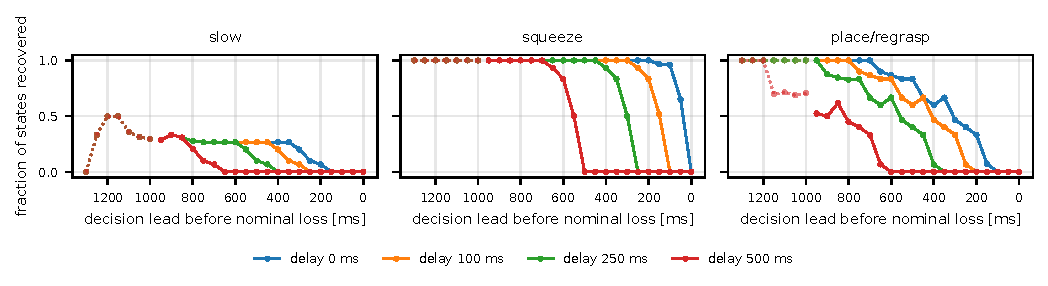
\includegraphics[width=\textwidth]{figures/fig_frontier.pdf}
\caption{\textbf{Recovery frontiers} (test episodes that nominal continuation loses; 637 decision states): fraction of states from which each remedy completes the task, versus decision lead before nominal loss, per response delay. Deadlines are remedy-specific and shift by roughly the delay. \remedy{slow} never exceeds one third because most losses are triggered by the push, not by transport acceleration. \remedy{place/regrasp} is non-monotone (recovery islands), so a single ``time-to-failure'' deadline would misdescribe it.}
\label{fig:frontier}
\end{figure*}

\section{Results}
\subsection{Remedy-specific deadlines}
Fig.~\ref{fig:frontier} shows recoverability from privileged branch labels. Using a 50\% recovery chance as the deadline, \remedy{squeeze} needs a decision lead of 50/150/300/550~ms at delays 0/100/250/500~ms, and \remedy{place/regrasp} 350/450/600/850~ms. The two deadlines differ by about 300~ms at every delay because the regrasp sequence itself takes time during which the object continues to slip. \remedy{slow} completes at most 33\% of lost states: 77 of the 100 nominal losses begin at or after the push, which slowing does nothing to counter. The oracle completes 100\% of test episodes at every delay by intervening in 31.9\% (median lead 1.05~s), so under this grid \emph{every} nominal loss was physically recoverable; what separates deployable supervisors from the oracle is knowing when and what to fire from stale, non-privileged evidence.

\subsection{Supervisors across the timing grid}
\begin{figure*}[t]
\centering
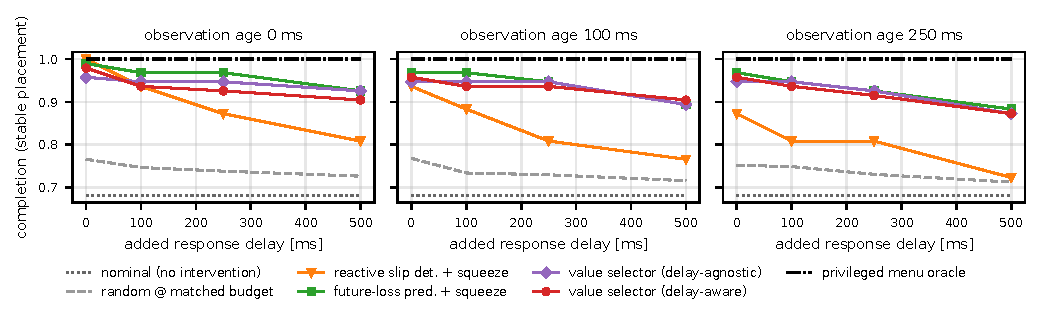
\includegraphics[width=\textwidth]{figures/fig_grid.pdf}
\caption{Closed-loop completion on 94 held-out episodes per cell. The reactive detector degrades steeply with both evidence age and delay; anticipatory supervisors degrade gently and track each other. Nominal completion is 0.68; random intervention at the same budget reaches 0.74.}
\label{fig:grid}
\end{figure*}

\begin{table}[t]
\caption{Pooled over the 12 timing cells (94 test episodes each). Gain is the paired completion difference versus nominal with 95\% bootstrap CI. Rate is the fraction of episodes with an intervention; rescue is the fraction of nominal losses converted to completion.}
\label{tab:main}
\centering
\footnotesize
\setlength{\tabcolsep}{3.5pt}
\begin{tabular}{@{}lcccc@{}}
\toprule
Supervisor & Compl. & Gain [95\% CI] & Rate & Rescue \\
\midrule
Nominal & .681 & -- & .00 & .00 \\
Random @ budget & .739 & +.058 [.044, .073] & .42 & .19 \\
Reactive slip + squeeze & .852 & +.171 [.149, .193] & .43 & .54 \\
Future loss + squeeze & \textbf{.946} & +.265 [.240, .292] & .48 & .83 \\
Value, delay-agnostic & .934 & +.253 [.228, .279] & .45 & .79 \\
Value, delay-aware & .930 & +.249 [.225, .275] & .42 & .78 \\
Oracle (privileged) & 1.000 & +.319 [.292, .348] & .32 & 1.00 \\
\bottomrule
\end{tabular}
\end{table}

Fig.~\ref{fig:grid} and Table~\ref{tab:main} give the main comparison. Every supervisor improves on nominal; random intervention at the same budget gains only 5.8 points, so intervention frequency does not explain the gains. The reactive slip detector is perfect with fresh evidence and no delay (1.00) but falls to 0.72 at 250~ms age and 500~ms delay: 28 points across the grid. Anticipatory supervisors span 11 points (future-loss 0.99$\to$0.88; delay-aware value 0.98$\to$0.87) because they fire with a median lead of 0.8--0.9~s versus 0.35~s, inside the \remedy{squeeze} deadline even at 500~ms delay. Age costs less than delay at every operating point.

\subsection{Does latency-conditioning help?}
It changes behaviour. The delay-aware selector reduces its intervention rate monotonically with delay (0.48$\to$0.37) while the delay-agnostic selector's rate is constant by construction, and with 250~ms-old evidence it shifts its menu toward \remedy{place/regrasp} (22 of 44 interventions at zero delay, 17 of 36 at 500~ms, versus 13 of 43 for the agnostic model), i.e.\ it prefers the slower but more decisive remedy when the evidence is stale. It does not complete more tasks: pooled paired differences are $-0.4$ points versus the agnostic selector (CI $[-1.0,+0.3]$) and $-1.6$ points versus future-loss~+~\remedy{squeeze} (CI $[-2.4,-0.9]$). Giving every learned supervisor a latency-tuned operating point (one validation threshold per cell) does not change this: $-0.6$ [$-1.3$, $0.0$] and $-0.4$ [$-1.3$, $+0.5$]. Realised test rates exceeded the 40\% validation budget by 2--8 points, which we report rather than re-tune. Fig.~\ref{fig:budget} shows the full budget--completion curves: the anticipatory supervisors coincide up to 60\% intervention, and all reach the oracle only at 100\%, i.e.\ \emph{squeeze everything}.

\begin{figure}[t]
\centering
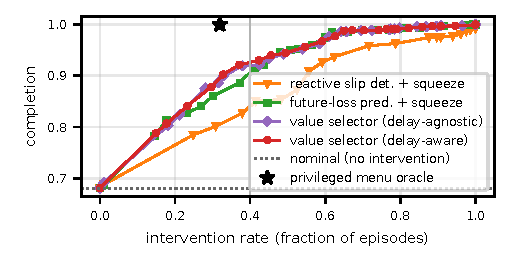
\includegraphics[width=0.82\columnwidth]{figures/fig_budget.pdf}
\caption{Completion versus intervention rate (test, pooled) as each threshold is swept. Vertical line: validation budget; star: oracle.}
\label{fig:budget}
\end{figure}

\subsection{Feedback-null controls}
With the delay-aware selector frozen, we replaced its observation features at test time while keeping timing features and labels intact. Frozen observations (the first decision state repeated) drop pooled completion from 0.930 to 0.810 ($-12.0$ points, CI $[-13.9,-10.2]$); observations swapped from another episode at the same step give 0.838 ($-9.2$, $[-11.5,-6.9]$); training-mean masking gives 0.894 ($-3.6$, $[-5.4,-1.7]$), but degenerately: with constant observations the decision depends only on the timing inputs, and the selector squeezes every episode at the first eligible step in eight cells and none in the other four (67\% overall). The selector's gain therefore depends on informative, episode-specific observations; the timing inputs alone do not produce it.

\subsection{Held-out friction band}
Re-splitting so that friction $\in[0.50,0.58]$ (64 acquired episodes) is never seen in training or validation: nominal 0.562; future-loss~+~\remedy{squeeze} 0.814; delay-agnostic 0.829; delay-aware 0.812; oracle 1.000 at 44\% intervention. The ordering is unchanged; the aware-minus-agnostic difference is $-1.7$ points (CI $[-2.9,-0.7]$). Completion is lower than on the random split because this band is where the nominal grasp is most often marginal.

\subsection{Cost}
Per-decision inference on one Apple M4 core (unoptimised scikit-learn): median 2.9--3.3~ms (p95 7~ms) for the detectors, 11.6~ms (p95 22~ms) for the value selectors; all fit inside one 50~ms control step. Energy is not measured or claimed.

\section{Discussion and limits}
\label{sec:limits}
Three readings follow. (i) Recoverability is not the bottleneck here: the oracle completes everything at 500~ms delay. The bottleneck is the \emph{evidence race}---whether non-privileged observations identify the episode before the remedy's deadline minus the delay. (ii) Because \remedy{squeeze} is the fastest remedy and, within its deadline, almost always sufficient, the value of the richer menu collapses to ``squeeze early enough'', which a future-loss predictor already does. The delay-aware model learns the right qualitative behaviour (fewer, differently chosen interventions as delay grows) without a measurable completion benefit at this budget and sample size. (iii) Reactive detection, which many systems deploy, is the one design that latency breaks.

The claims are bounded by: simulation only, with soft contacts standing in for real friction; one rigid cube; an ideal Cartesian carrier; a scripted controller and remedies; deterministic physics with a single exogenous push, so paired outcomes are binary rather than calibrated probabilities; fixed synthetic delays rather than measured latency traces; proprioception and wrist force only; 94 test episodes, leaving differences below about two points unresolved; and a menu in which squeezing is cheap---objects with a crush limit, or a gripper already at its force bound, would change the frontier and could restore the value of a menu-aware selector. Those are the conditions under which we expect the latency-conditioned model to matter, and they are the next experiment: a hidden fragility limit, a weaker squeeze, measured latency traces, more geometries, then matched (not counterfactual-exact) blocks on a physical arm. Code, branch tables, the report containing every number above, lookup-verification records and this manuscript are in the repository named in the title block.

\begin{thebibliography}{9}
\bibitem{faildetect} C.~Xu \emph{et al.}, ``Can we detect failures without failure data? (FAIL-Detect),'' \emph{RSS}, 2025.
\bibitem{safe} Q.~Gu \emph{et al.}, ``SAFE: Multitask failure detection for vision-language-action models,'' \emph{NeurIPS}, 2025.
\bibitem{rtc} K.~Black, M.~Y.~Galliker, S.~Levine, ``Real-time execution of action chunking flow policies,'' Physical Intelligence, 2025.
\bibitem{reflex} ``Reflex / ReflexBench: manipulation under configurable inference latency,'' arXiv:2608.14379, 2026.
\bibitem{roborecover} ``RoboRecover: recovery from execution-induced intermediate states,'' arXiv:2609.28952, 2026.
\bibitem{kintsugi} ``Kintsugi-VLA: expert-relative recoverability via state restoration and branching,'' arXiv:2609.31048, 2026.
\bibitem{intervenesim} E.~Villalovoz, ``InterveneSim-Value,'' GitHub repository \mbox{ethanvillalovoz/intervenesim}, 2026.
\bibitem{far} H.~Tan, ``Failure recovery in remote VLA deployment,'' GitHub repository \mbox{HyuanTan/lerobot\_far}, 2026.
\bibitem{slipbound} F.~Veiga, B.~Edin, J.~Peters, ``Grip stabilization of novel objects using slip prediction,'' \emph{IEEE T-Haptics}, 11(4), 2018.
\bibitem{feeling} R.~Calandra \emph{et al.}, ``The feeling of success: does touch sensing help predict grasp outcomes?'' \emph{CoRL}, 2017.
\end{thebibliography}

\end{document}
